\documentclass[12pt]{article}
\usepackage[utf8]{inputenc}
\usepackage{float}
\usepackage{amsmath}


\usepackage[hmargin=3cm,vmargin=6.0cm]{geometry}
%\topmargin=0cm
\topmargin=-2cm
\addtolength{\textheight}{6.5cm}
\addtolength{\textwidth}{2.0cm}
%\setlength{\leftmargin}{-5cm}
\setlength{\oddsidemargin}{0.0cm}
\setlength{\evensidemargin}{0.0cm}

%misc libraries goes here
\usepackage{tikz}
\usetikzlibrary{automata,positioning}

\begin{document}

\section*{Student Information } 
%Write your full name and id number between the colon and newline
%Put one empty space character after colon and before newline
Full Name : Bilal Özlü \\
Id Number : 1942614 \\

% Write your answers below the section tags
\section*{Answer 1}

\subsection*{a.}
(a)((a+c)*(b)(a+c)*(b)(a+c)*)(cc) \\
\subsection*{b.}
(b+c)(bb+bc+cb+cc)*(a)(bb+bc+cb+cc)* + (bb+bc+cb+cc)*(a)(b+c)(bb+bc+cb+cc)* \\
\subsection*{c.}
(a*)((b$^+$a$^+$b$^+$a$^+$)*)(b*) \\
\section*{Answer 2}

\subsection*{a.}
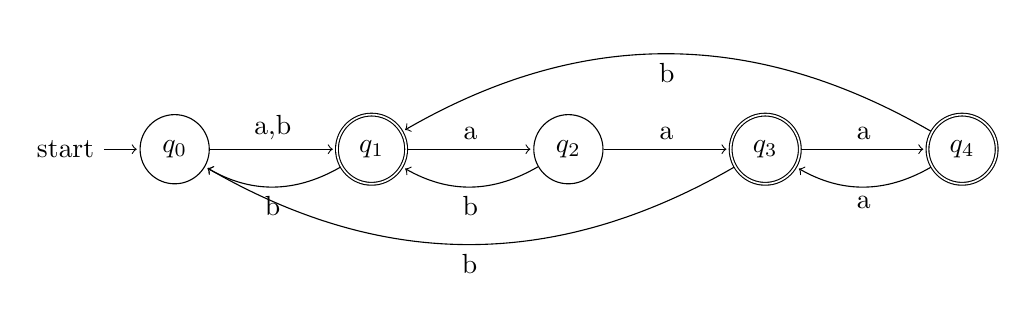
\begin{tikzpicture}[shorten >=1pt,node distance=2.5cm,on grid,auto]
\node[state,initial] (q_0) {$q_0$};
\node[state,accepting] (q_1) [right=of q_0] {$q_1$};
\node[state] (q_2) [right=of q_1] {$q_2$};
\node[state,accepting] (q_3) [right=of q_2] {$q_3$};
\node[state,accepting] (q_4) [right=of q_3] {$q_4$};
\path[->]
(q_0) edge node {a,b} (q_1) 
(q_1) edge node {a} (q_2) edge [bend left] node {b} (q_0)
(q_2) edge node {a} (q_3) edge [bend left] node {b} (q_1)
(q_3) edge node {a} (q_4) edge [bend left] node {b} (q_0)
(q_4) edge [bend left] node {a} (q_3) edge [bend right] node {b} (q_1);
\end{tikzpicture}
\subsection*{b.}
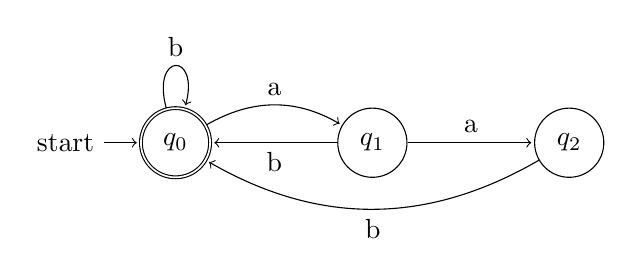
\begin{tikzpicture}[shorten >=1pt,node distance=2.5cm,on grid,auto]
\node[state,initial, accepting] (q_0) {$q_0$};
\node[state] (q_1) [right=of q_0] {$q_1$};
\node[state] (q_2) [right=of q_1] {$q_2$};
\path[->]
(q_0) edge [bend left] node {a} (q_1) edge [loop above] node {b} (q_0)
(q_1) edge node {a} (q_2) edge node {b} (q_0)
(q_2) edge [bend left] node {b} (q_0);
\end{tikzpicture}

\section*{Answer 3}
It is not. $\lbrace$01$\rbrace$,$\lbrace$0011$\rbrace$... are regular since they contain only a string, \\
however the infinite union is the set of $\lbrace$0$^x$1$^x$ $\vert$ x$\geq$0$\rbrace$ \\
and it is not regular obviously by Pumping Lemma. \\
Hence the infinite unions are not closed for the family of regular languages. \\

\section*{Answer 4}
Let's say L = $\lbrace$ a$^i$b$^j$c$^{2j}$ $\vert$ i$\geq$0 , j$\geq$0 $\rbrace$. \\
Since L is infinite, we can apply Pumping Lemma. \\
Let m be the integer in the Pumping Lemma. \\
Pick a string w such that w $\in$ L and length $\vert$w$\vert$ $\geq$ m. \\
We pick w = a$^m$b$^m$c$^{2m}$. Let's write a$^m$b$^m$c$^{2m}$ = xyz. \\
From the pumping lemma, it must be length $\vert$ y z $\vert$ $\leq$ m , $\vert$ y $\vert$ $\geq$ 1 \\
.$\hspace{41pt}$m$\hspace{21pt}$m$\hspace{41pt}$2m \\	
xyz = $\overbrace{aa...a}$ $\overbrace{bb...b}$ $\overbrace{cc...cc...cc...cc...c}$ \\
xyz = $\underbrace{aa...abb...bcc...cc...cc}$ $\underbrace{c...c}$ $\underbrace{c...c}$ \\
.$\hspace{81pt}$x$\hspace{59pt}$y$\hspace{21pt}$z \\
Thus  y=c$^k$, k$\geq$1. \\
From the Pumping Lemma, xy$^i$z = xz $\in$ L, i=0,1,2... So, xy$^0$z = xz $\in$ L. \\
.$\hspace{36pt}$m$\hspace{20pt}$m$\hspace{28pt}$2m-k \\
xz = $\overbrace{aa...a}$ $\overbrace{bb...b}$ $\overbrace{cc...cc...cc...c}$ \\
xz = $\underbrace{aa...abb...bcc...cc...cc}$ $\underbrace{c...c}$ \\
.$\hspace{75pt}$x$\hspace{60pt}$z \\
a$^m$ b$^m$ c$^{2m-k}$ $\in$ L, k$\geq$1 \\
But, L=$\lbrace$ a$^i$b$^j$c$^{2j}$ $\vert$ i$\geq$0 , j$\geq$0 $\rbrace$ ,therefore a$^m$ b$^m$ c$^{2m-k}$ $\in$ L is not true! \\
And so L is not regular. \\

\section*{Answer 5}
Proof1] \\
\\
Regular languages are closed under set difference. \\
Because L1 - L2 = L1 $\cap$ $\overline{L2}$ = $\overline{ \overline{L1} \cup L2}$. \\
And regular languages are closed under union(ii) and complementation(i). \\
$\overline{L1}$ and L2 is regular. \\
$\overline{ \overline{L1} \cup L2}$ is also regular. \\
Hence, L1 - L2 is regular. For every pair of regular languages L1 and L2, L1 - L2 is also regular. \\
And the family of regular languages is closed under set difference. \\
\\
i) Complement of a language L is $\sum$* – L (for an alphabet $\sum$. And $\sum$* contains L) \\
Since $\sum$* is regular, the complement of a regular language is always regular. \\
\\
ii)Let Lx and Ly be the languages of regular expressions R1 and R2,respectively. \\
Then R1 + R2 is a regular expression whose language is Lx $\cup$ Ly. \\ 
If Lx and Ly are regular, Lx $\cup$ Ly is also regular. So regular languages are closed under union. \\
\\
Proof2] \\
\\
Let L1 and L2 be DFA’s languages. \\
Let L3 = L1 - L2 \\
The final states of L3 will be the pairs where L1-state is final but L2-state is not. \\
And it is also a DFA language, so it is a regular language always. \\  

\section*{Answer 6}
\begin{tikzpicture}[shorten >=1pt,node distance=2.5cm,on grid,auto]
\node[state,initial] (x_0) {$x_0$};
\node[state,accepting] (x_1) [right=of x_0] {$x_1$};
\node[state] (x_2) [right=of x_1] {$x_2$};
\node[state,accepting] (x_3) [right=of x_2] {$x_3$};
\node[state] (x_4) [right=of x_3] {$x_4$};
\node[state,accepting] (x_5) [below=of x_2] {$x_5$};
\node[state,accepting] (x_6) [below=of x_5] {$x_6$};
\node[state] (x_7) [below=of x_6] {$x_7$};
\node[state,accepting] (x_8) [right=of x_7] {$x_8$};
\node[state,accepting] (x_9) [right=of x_8] {$x_9$};
\path[->]
(x_0) edge node {a} (x_1) edge [loop above] node {b} (x_0)
(x_1) edge [bend left] node {a} (x_0) edge node {b} (x_2)
(x_2) edge node {a} (x_3) edge node {b} (x_5)
(x_3) edge node {a} (x_4) edge [bend left] node {b} (x_2)
(x_4) edge [loop right] node {a} (x_4) edge [loop above] node {b} (x_4)
(x_5) edge node {a} (x_6) edge [loop left] node {b} (x_5)
(x_6) edge [bend left] node {a} (x_1) edge node {b} (x_7)
(x_7) edge [bend left] node {a} (x_1) edge node {b} (x_8)
(x_8) edge node {a} (x_9) edge [loop above] node {b} (x_8)
(x_9) edge [loop right] node {a} (x_9) edge [bend left] node {b} (x_7)
; 
\end{tikzpicture} \\
x0 = q$_0$ \\
x1 = q$_1$,q$_2$ \\
x2 = q$_3$ \\
x3 = q$_2$ \\
x4 = - (trap)\\
x5 = q$_1$,q$_3$\\
x6 = q$_0$,q$_2$\\
x7 = q$_0$,q$_3$\\
x8 = q$_0$,q$_1$,q$_3$\\
x9 = q$_0$,q$_1$,q$_2$\\
\\
There is no unreachable state, it can be seen on the graph clearly. \\
And also there is no non-distinguishable state, it can be seen in the table below. \\
Hence, this is the minimal DFA. It cannot be minimized anymore.  \\
.$\hspace{16pt}$a$\hspace{14pt}$b \\
x0: x1 x0 \\
x1: x0 x2  \\
x2: x3 x5  \\
x3: x4 x2  \\
x4: x4 x4  \\
x5: x6 x5  \\
x6: x1 x7  \\
x7: x1 x8  \\
x8: x9 x8  \\
x9: x9 x7  \\

\end{document}
